% Provenance (never printed): old premiere S / seconde material on minerals and
% rocks (identifying minerals in hand specimen, the silicates, the minerals of
% granite, basalt and peridotite, thin sections in polarised light).
% Element fractions and rock densities from figdata/grade-11/mineral_density.py
% (Rudnick and Gao 2014 bulk crust; webmineral mean densities). Mineral, crystal,
% rock families and the Mohs scale are Book 1's (grade 6): recalled, not defined.
% Felsic and mafic belong to g11.08: not used here.
\chapter{Mineralen}\label{ch:g11:minerals}

Raap een granieten kiezel op en bekijk hem door een loep. Het is niet één
stof maar een mozaïek van korrels die in elkaar grijpen: grijze korrels, glazig en
bijna doorzichtig; roze korrels, blokvormig, waarvan de breukvlakken in het licht
oplichten wanneer je de kiezel draait; kleine zwarte schilfers die een mespunt in
dunne blaadjes loswipt. Elk soort korrel is een mineraal. Dit hoofdstuk laat zien hoe
een geoloog ze uit elkaar houdt, waarom bijna allemaal uit silicium en zuurstof
zijn opgebouwd, hoe ze de gesteenten vormen die we tot nu toe hebben gezien --- graniet,
basalt, \omterm{def:g11:ocean-ridges:peridotite}{peridotiet} --- en hoe een plakje gesteente dat dunner is dan een haar, in
gepolariseerd licht bekeken, ze allemaal tegelijk laat zien.

\begin{omfigure}
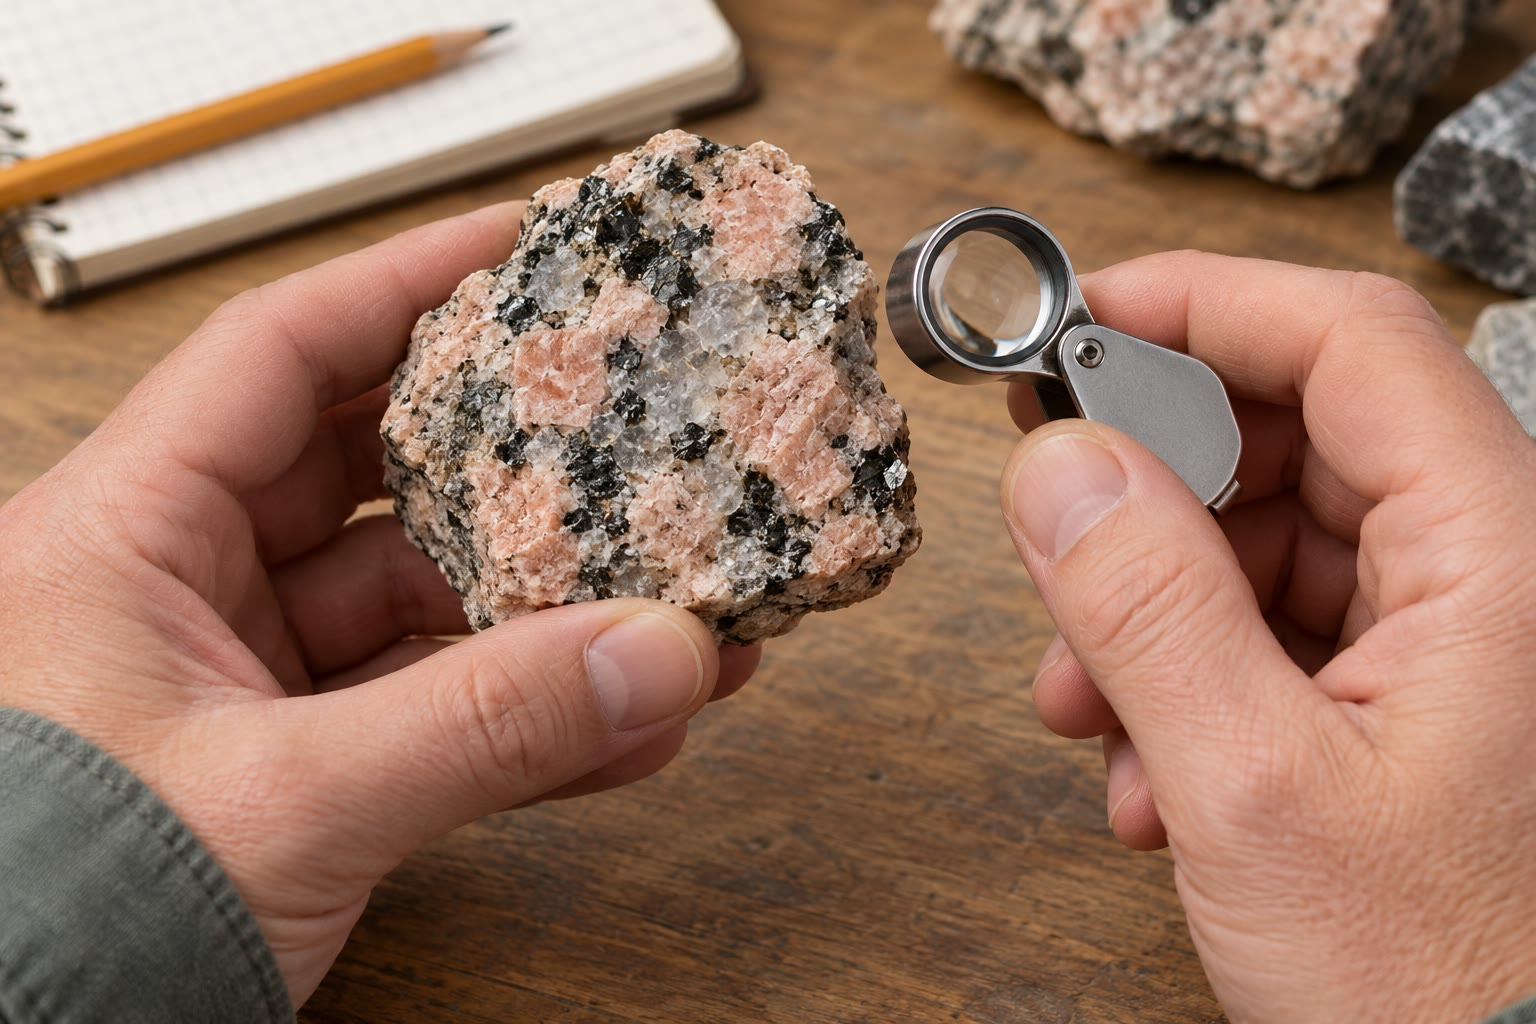
\includegraphics[width=0.62\linewidth]{images/book2/ai/g11-geologist-hand-lens.jpg}

{\small Een graniet onderzocht met een loep: het eerste hulpmiddel om
mineralen uit elkaar te houden. (AI-illustratie.)}
\end{omfigure}

\begin{recall}
Een mineraal is een natuurlijke vaste stof, niet gemaakt door levende wezens, met een
vaste samenstelling en atomen die regelmatig zijn gerangschikt; een gesteente bestaat uit één
of meer mineralen. Graniet bestaat vooral uit veldspaat, kwarts en mica.
Gesteenten vallen in drie families: stollingsgesteenten, sedimentaire en metamorfe gesteenten. De
hardheid van een mineraal is hoe goed het weerstand biedt tegen krassen, gerangschikt van 1
(talk) tot 10 (diamant) op de schaal van Mohs; orthoklaas-veldspaat heeft 6 en kwarts
7, terwijl een glasplaatje ongeveer 5.5 heeft en een stalen spijker ongeveer 6.5 (Boek 1,
jaar 6). De dichtheid van een lichaam is zijn massa gedeeld door zijn volume
(natuurkunde). Een verbinding wordt beschreven door een formule die haar atomen telt; in een
vaste stof uit ionen zijn de positieve en negatieve ladingen in evenwicht (scheikunde).
\omterm{def:g11:ocean-ridges:peridotite}{Peridotiet} vormt de mantel; \omterm{def:g11:ocean-ridges:gabbro}{gabbro} en basalt vormen de \omterm{def:g11:ocean-ridges:oceanic-lithosphere}{oceanische korst}
(\cref{ch:g11:ocean-ridges}).
\end{recall}
% ledger: usgs:mineral-rock, nps:granite-minerals, nps:mohs-ladder, nps:mohs-testers

\section{Mineralen uit elkaar houden}

Een mineraal heeft een vaste samenstelling en een regelmatige rangschikking van atomen. Beide
zijn aan de buitenkant te zien: in de vorm van zijn kristallen, de manier waarop het breekt, de
manier waarop het licht weerkaatst, zijn hardheid en zijn dichtheid. Geen van deze eigenschappen
is op zich genoeg; samen identificeren ze de gewone mineralen in een handstuk,
met als enige hulpmiddelen een loep, een stalen spijker en een glasplaatje.

\paragraph{Vorm.} Een kristal dat vrij is gegroeid, in een holte of in een vloeistof,
krijgt een vorm die de rangschikking van zijn atomen weerspiegelt.

\begin{definition}[Habitus]\label{def:g11:minerals:habit}
De \emph{habitus}\index{habitus (van een kristal)} van een mineraal is de algemene vorm
die zijn kristallen aannemen: kubisch, tabulair (plat, als een tablet), prismatisch
(langwerpig, als een prisma), bladvormig, naaldvormig, enzovoort.
\end{definition}
% ledger: tulane:physprop

Kwarts groeit als zeszijdige prisma's die in punten uitlopen; biotiet als platte
zeszijdige plaatjes (foto's hieronder). In de meeste gesteenten zijn de korrels echter
tegen elkaar aan gegroeid en hebben ze geen eigen vlakken: de \omterm{def:g11:minerals:habit}{habitus} zegt dan weinig,
en de andere eigenschappen nemen het over.
% ledger: photo:g11-quartz, photo:g11-biotite

\paragraph{Kleur en glans.} Kleur is het eerste wat je ziet, en het
minst betrouwbaar. Een spoor van een ander element is genoeg om haar te veranderen: kwarts
kan helder, wit, zwart, roze, blauw of paars zijn. Een paar mineralen variëren
daarentegen nauwelijks: olivijn is bijna altijd groen. Hoe een mineraal
licht weerkaatst, is een betere gids.
% ledger: tulane:physprop

\begin{definition}[Glans]\label{def:g11:minerals:lustre}
De \emph{glans}\index{glans} van een mineraal is zijn uiterlijk in weerkaatst
licht. Ze is \emph{metaalachtig} wanneer het mineraal glanst als een metaal, en
anders niet-metaalachtig: \emph{glasachtig} (zoals kwarts), parelmoerachtig,
harsachtig, enzovoort.
\end{definition}
% ledger: tulane:physprop

\paragraph{De manier waarop het breekt.} Sla op een kristal en het breekt. Waar de
bindingen tussen zijn atomen langs bepaalde vlakken zwakker zijn, splijt het daarlangs,
keer op keer, in platte glanzende vlakken; waar geen vlak zwakker is
dan een ander, breekt het langs een willekeurig oppervlak.

\begin{definition}[Splijting; breuk]\label{def:g11:minerals:cleavage}
\emph{Splijting}\index{splijting (van een mineraal)} is de neiging van een mineraal
om te breken langs platte vlakken, evenwijdig aan richtingen waarin de bindingen
tussen zijn atomen zwakker zijn. \emph{Breuk}\index{breuk (van een mineraal)}
is breken langs onregelmatige oppervlakken, in een mineraal zonder
zwaktevlak; een breuk met gladde gebogen oppervlakken, zoals gebroken glas, heet
\emph{schelpvormig}.
\end{definition}
% ledger: tulane:physprop

Een mineraal kan één \omterm{def:g11:minerals:cleavage}{splijtrichting} hebben, twee, drie of geen. Mica's hebben er één, perfect:
ze laten zich in blaadjes afpellen. Veldspaten hebben er twee. Kwarts heeft er geen: het breekt met een
schelpvormige breuk, waardoor het meteen te onderscheiden is van een veldspaat met dezelfde grijze
of witte kleur. De hoek tussen twee \omterm{def:g11:minerals:cleavage}{splijtrichtingen} ligt vast door de rangschikking
van de atomen, en kan worden gemeten op een gebroken korrel of een doorsnede: de twee
\omterm{def:g11:minerals:cleavage}{splijtrichtingen} van een pyroxeen snijden elkaar onder ongeveer \ang{87} en \ang{93}, bijna een rechte
hoek; die van een amfibool onder ongeveer \ang{56} en \ang{124}. Pyroxenen en
amfibolen zijn vaak donker en lijken op elkaar; hun splijthoeken onderscheiden ze.
% ledger: wm:densities (quartz conchoidal; orthoclase two cleavages; biotite one), tulane:cleavage-angles

\begin{omfigure}
\begin{tikzpicture}[font=\footnotesize]
  % pyroxene: octagonal cross-section, cleavage traces at 46.5 and 133.5 degrees (87/93)
  \begin{scope}
    \coordinate (p1) at (1,0.4); \coordinate (p2) at (0.431,1); \coordinate (p3) at (-0.431,1);
    \coordinate (p4) at (-1,0.4); \coordinate (p5) at (-1,-0.4); \coordinate (p6) at (-0.431,-1);
    \coordinate (p7) at (0.431,-1); \coordinate (p8) at (1,-0.4);
    \begin{scope}[scale=1.5]
      \fill[black!72!green!40] (1,0.4) -- (0.431,1) -- (-0.431,1) -- (-1,0.4) -- (-1,-0.4) -- (-0.431,-1) -- (0.431,-1) -- (1,-0.4) -- cycle;
      \clip (1,0.4) -- (0.431,1) -- (-0.431,1) -- (-1,0.4) -- (-1,-0.4) -- (-0.431,-1) -- (0.431,-1) -- (1,-0.4) -- cycle;
      \foreach \s in {-5,...,5} {
        \draw[white!85!black, line width=0.5pt] ($(136.5:\s*0.24)+(46.5:-3)$) -- ($(136.5:\s*0.24)+(46.5:3)$);
        \draw[white!85!black, line width=0.5pt] ($(223.5:\s*0.24)+(133.5:-3)$) -- ($(223.5:\s*0.24)+(133.5:3)$);}
      \draw[black!80, line width=0.9pt] (46.5:-3) -- (46.5:3); \draw[black!80, line width=0.9pt] (133.5:-3) -- (133.5:3);
    \end{scope}
    \draw[black!70, line width=0.7pt, scale=1.5] (1,0.4) -- (0.431,1) -- (-0.431,1) -- (-1,0.4) -- (-1,-0.4) -- (-0.431,-1) -- (0.431,-1) -- (1,-0.4) -- cycle;
    \draw[omProp, line width=1pt] (46.5:0.75) arc[start angle=46.5, end angle=133.5, radius=0.75];
    \draw[omDef, line width=1pt] (133.5:0.5) arc[start angle=133.5, end angle=226.5, radius=0.5];
    \node[fill=white, inner sep=1pt, text=omProp!80!black] at (90:0.98) {\ang{87}};
    \node[fill=white, inner sep=1pt, text=omDef] at (180:0.82) {\ang{93}};
    \node[anchor=north, align=center] at (0,-1.7) {\strut\textbf{pyroxeen}\\splijting onder ongeveer \ang{87} en \ang{93}};
  \end{scope}
  % amphibole: elongated hexagon, cleavage traces at 28 and 152 degrees (56/124 opening sideways)
  \begin{scope}[xshift=6.2cm]
    \begin{scope}[scale=1.5]
      \fill[black!72!green!40] (1.6,0) -- (0.62,0.52) -- (-0.62,0.52) -- (-1.6,0) -- (-0.62,-0.52) -- (0.62,-0.52) -- cycle;
      \clip (1.6,0) -- (0.62,0.52) -- (-0.62,0.52) -- (-1.6,0) -- (-0.62,-0.52) -- (0.62,-0.52) -- cycle;
      \foreach \s in {-6,...,6} {
        \draw[white!85!black, line width=0.5pt] ($(118:\s*0.2)+(28:-4)$) -- ($(118:\s*0.2)+(28:4)$);
        \draw[white!85!black, line width=0.5pt] ($(242:\s*0.2)+(152:-4)$) -- ($(242:\s*0.2)+(152:4)$);}
      \draw[black!80, line width=0.9pt] (28:-4) -- (28:4); \draw[black!80, line width=0.9pt] (152:-4) -- (152:4);
    \end{scope}
    \draw[black!70, line width=0.7pt, scale=1.5] (1.6,0) -- (0.62,0.52) -- (-0.62,0.52) -- (-1.6,0) -- (-0.62,-0.52) -- (0.62,-0.52) -- cycle;
    \draw[omProp, line width=1pt] (-28:0.75) arc[start angle=-28, end angle=28, radius=0.75];
    \draw[omDef, line width=1pt] (28:0.42) arc[start angle=28, end angle=152, radius=0.42];
    \node[fill=white, inner sep=1pt, text=omProp!80!black] at (0:1.02) {\ang{56}};
    \node[fill=white, inner sep=1pt, text=omDef] at (90:0.6) {\ang{124}};
    \node[anchor=north, align=center] at (0,-1.7) {\strut\textbf{amfibool}\\splijting onder ongeveer \ang{56} en \ang{124}};
  \end{scope}
\end{tikzpicture}

{\small Doorsneden van een pyroxeenkristal (links) en een amfiboolkristal
(rechts), dwars op hun lengte gesneden (een tekening). De dunne lijnen zijn de sporen
van de twee \omterm{def:g11:minerals:cleavage}{splijtrichtingen}, waarvan er twee dikker zijn getekend waar de hoeken worden afgelezen;
de hoeken ertussen, bijna recht in het pyroxeen, veel opener en veel scherper in het amfibool, onderscheiden twee
verder gelijkende donkere mineralen.}
\end{omfigure}
% ledger: tulane:cleavage-angles

\paragraph{Hardheid en dichtheid.} Hardheid, gezien in Boek 1, onderscheidt
mineralen die op elkaar lijken: kwarts (7) krast glas en wordt niet gekrast door
een stalen spijker; een veldspaat (6) krast ook glas, maar de spijker krast hem.
Dichtheid is de laatste aanwijzing. In de hand kun je een korrel niet wegen, maar een
handstuk van één mineraal wel, en de gewone mineralen van gesteenten beslaan een smal
bereik, van ongeveer \qty{2.6}{g/cm^3} tot ongeveer \qty{3.4}{g/cm^3} (diagram hieronder):
de lichtste zijn rijk aan silicium, aluminium, natrium en kalium, de
dichtste aan ijzer en magnesium.
% ledger: nps:mohs-ladder, nps:mohs-testers, wm:densities

\begin{method}[Een mineraal in een handstuk identificeren]\label{met:g11:minerals:identify}
\begin{enumerate}
  \item Bekijk de vorm van de korrel of het kristal (\omterm{def:g11:minerals:habit}{habitus}), zijn kleur --- alleen
        als hint --- en zijn \omterm{def:g11:minerals:lustre}{glans}.
  \item Zoek naar \omterm{def:g11:minerals:cleavage}{splijting}: platte glanzende vlakken die samen het licht
        vangen wanneer je het handstuk draait. Tel de \omterm{def:g11:minerals:cleavage}{splijtrichtingen}
        en schat de hoek ertussen; als er geen is, beschrijf dan de
        breuk.
  \item Test de hardheid met referentievoorwerpen: een glasplaatje (ongeveer
        5.5) en een stalen spijker (ongeveer 6.5).
  \item Als het handstuk uit één mineraal bestaat, vergelijk dan zijn dichtheid met de
        dichtheden van de kandidaten.
  \item Besluit op grond van de combinatie van eigenschappen, nooit op grond van één alleen.
\end{enumerate}
\end{method}
% ledger: nps:mohs-testers

\begin{example}[Kwarts of veldspaat?]
Twee grijswitte korrels in een graniet. De eerste toont geen plat vlak, alleen
gladde gebogen breuken, en de stalen spijker laat er geen spoor op na: schelpvormige
breuk en een hardheid boven 6.5, het is kwarts (7). De tweede breekt in
platte glanzende vlakken in twee richtingen en wordt door de spijker gekrast, hoewel
hij glas krast: twee \omterm{def:g11:minerals:cleavage}{splijtrichtingen} en een hardheid tussen 5.5 en 6.5, het is
een veldspaat (6).
\end{example}
% ledger: wm:densities, nps:mohs-ladder, nps:mohs-testers

\begin{omfigure}
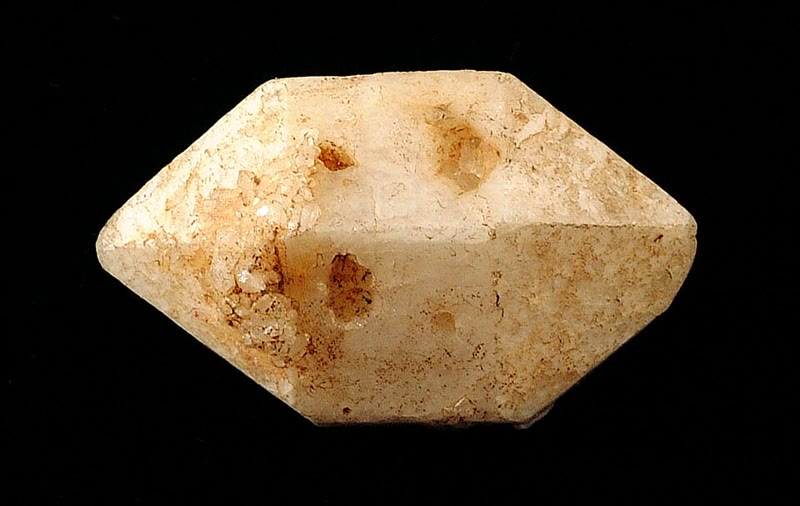
\includegraphics[height=2.75cm]{images/book2/g11-geodil-quartz.jpg}\hfill
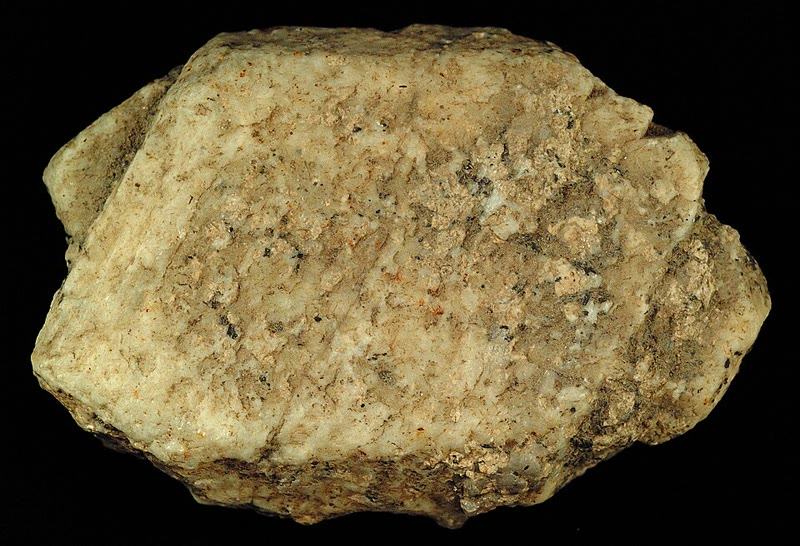
\includegraphics[height=2.75cm]{images/book2/g11-geodil-orthoclase.jpg}\hfill
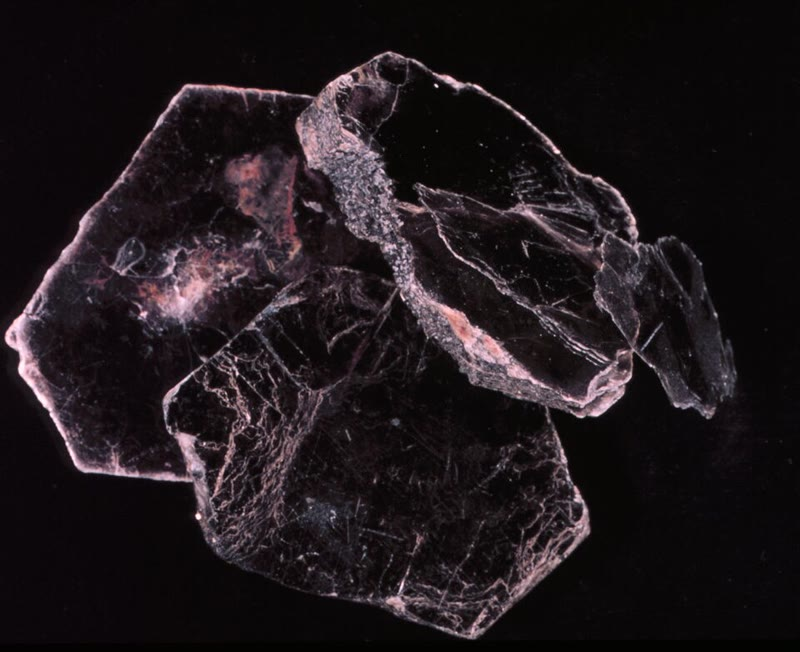
\includegraphics[height=2.75cm]{images/book2/g11-geodil-biotite.jpg}\hfill
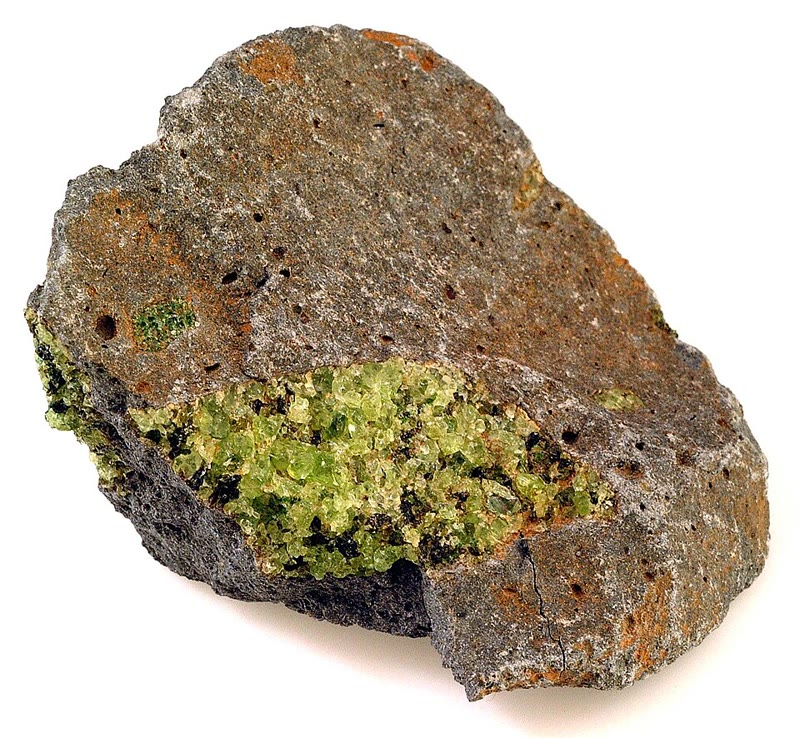
\includegraphics[height=2.75cm]{images/book2/g11-geodil-olivine.jpg}

{\small Vier gesteentevormende mineralen. Van links naar rechts: een kwartskristal,
een zeszijdig prisma dat aan beide uiteinden in een punt uitloopt, ongeveer \qty{5}{cm} lang; een
orthoklaas-veldspaat, twee kristallen die samen zijn gegroeid, ongeveer \qty{7}{cm};
zeszijdige plaatjes biotiet-mica, ongeveer \qty{6}{cm}, die langs hun enige \omterm{def:g11:minerals:cleavage}{splijtrichting} in dunne
blaadjes splijten; groene korrels olivijn in een basalt.
Foto's Shannon Heinle, Darla Sondrol, Dexter Perkins en Nessa Eull,
Geology Digital Image Library (CC0).}
\end{omfigure}
% ledger: photo:g11-quartz, photo:g11-orthoclase, photo:g11-biotite, photo:g11-olivine

\section{Silicaten}

\paragraph{Twee elementen maken de korst.} De chemische samenstelling van de
continentale korst is bekend uit de analyses van vele gesteenten, opgegeven als
percentages oxiden: ongeveer \qty{60.6}{\percent} \ce{SiO2},
\qty{15.9}{\percent} \ce{Al2O3}, enzovoort. Daaruit, en uit de massa's van
de atomen, volgt de massa van elk element. Zuurstof maakt \qty{46}{\percent}
uit van de massa van de continentale korst en silicium \qty{28}{\percent}: twee
elementen, ongeveer drie kwart van de massa. Met zes metalen --- aluminium,
ijzer, calcium, magnesium, natrium en kalium --- maken ze meer dan
\qty{99}{\percent} ervan uit.
% ledger: rg14:crust, ciaaw:O, ciaaw:Si, ciaaw:Al, ciaaw:Fe, ciaaw:Ca, ciaaw:Mg, ciaaw:Na, ciaaw:K, ciaaw:Ti, ciaaw:Mn, ciaaw:P
% values (mineral_density.py): bulk_O 46.36, bulk_Si 28.30, O+Si 74.66, eight elements 99.43

\begin{omfigure}
\begin{tikzpicture}
\begin{axis}[omrecord, width=0.82\linewidth, height=5.6cm, ybar, bar width=14pt,
  ymin=0, ymax=55, xtick=data, enlarge x limits=0.06,
  xticklabels from table={figdata/out/grade-11-mineral_density-elements.dat}{symbol},
  ylabel={aandeel in de massa (\unit{\percent})},
  nodes near coords, every node near coord/.append style={font=\scriptsize, /pgf/number format/.cd, fixed, precision=1},
  xmajorgrids=false]
% computed in figdata/grade-11/mineral_density.py; ledger: rg14:crust, ciaaw:*
\addplot[fill=omDef!55, draw=omDef] table[x expr=\coordindex, y=frac] {figdata/out/grade-11-mineral_density-elements.dat};
\end{axis}
\end{tikzpicture}

{\small De elementen van de continentale korst, als aandelen in haar massa,
berekend uit haar gemiddelde samenstelling in oxiden (Rudnick en Gao, 2014).
Zuurstof en silicium alleen maken ongeveer drie kwart van de massa uit.}
\end{omfigure}

\paragraph{De silicium-zuurstoftetraëder.} Een siliciumatoom is klein, en
er passen vier zuurstofatomen omheen, op de hoekpunten van een tetraëder, een piramide
met vier driehoekige zijvlakken. De groep bevat één siliciumion \ce{Si^4+} en
vier zuurstofionen \ce{O^2-}: hij draagt een lading van $4 - 4 \times 2 = -4$,
die andere ionen --- of andere tetraëders --- moeten compenseren.

\begin{definition}[Silicaat; silicium-zuurstoftetraëder]\label{def:g11:minerals:silicate}
De \emph{silicium-zuurstoftetraëder}\index{silicium-zuurstoftetraeder@silicium-zuurstoftetraëder} is
de groep \ce{SiO4} die wordt gevormd door één siliciumatoom en de vier zuurstofatomen
eromheen, op de hoekpunten van een tetraëder. Een
\emph{silicaat}\index{silicaat} is een mineraal dat is opgebouwd uit
silicium-zuurstoftetraëders, los of met elkaar verbonden via gedeelde hoekpunten.
\end{definition}
% ledger: tulane:silicates

Tetraëders verbinden zich door zuurstofatomen te delen: het hoekpunt van de ene tetraëder is het
hoekpunt van de volgende. Hoeveel hoekpunten elke tetraëder deelt, bepaalt de
structuur van het \omterm{def:g11:minerals:silicate}{silicaat}, en zijn formule.
\begin{itemize}
  \item \emph{Losse tetraëders}, die geen hoekpunt delen, bijeengehouden door
        metaalionen ertussen: olivijn, \ce{(Mg,Fe)2SiO4}.
  \item \emph{Enkele ketens}, waarin elke tetraëder twee hoekpunten deelt met zijn
        buren: de pyroxenen.
  \item \emph{Dubbele ketens}, twee enkele ketens zij aan zij verbonden, waarbij de
        tetraëders om beurten twee of drie hoekpunten delen: de amfibolen.
  \item \emph{Lagen}, waarin elke tetraëder drie hoekpunten deelt: de mica's,
        en de kleimineralen van bodems (\cref{ch:g10:soil-formation}).
  \item \emph{Raamwerken}, waarin elke tetraëder alle vier zijn hoekpunten deelt, in alle
        drie de richtingen van de ruimte: kwarts, \ce{SiO2}, en --- met aluminium
        op de plaats van een deel van het silicium --- de veldspaten.
\end{itemize}
% ledger: tulane:silicates

\begin{omfigure}
\begin{tikzpicture}[font=\footnotesize]
  % coordinates generated once by a small script (scratch, not kept): kagome net of side 0.62 cm,
  % a regular tetrahedron in perspective, and a framework piece of five tetrahedra (painter's order)
  % (a) one SiO4 tetrahedron, drawn in perspective; the silicon (black) at its centre
  \fill[omDef!12] (2.300,2.979) -- (1.927,1.372) -- (1.221,0.629) -- (3.752,0.820) -- cycle;
  \draw[densely dashed, omDef!60, line width=0.6pt] (2.300,2.979) -- (1.927,1.372);
  \draw[omDef!70!black, line width=0.6pt] (2.300,2.979) -- (1.221,0.629);
  \draw[omDef!70!black, line width=0.6pt] (2.300,2.979) -- (3.752,0.820);
  \draw[densely dashed, omDef!60, line width=0.6pt] (1.927,1.372) -- (1.221,0.629);
  \draw[densely dashed, omDef!60, line width=0.6pt] (1.927,1.372) -- (3.752,0.820);
  \draw[omDef!70!black, line width=0.6pt] (1.221,0.629) -- (3.752,0.820);
  \draw[black!55, line width=0.4pt] (2.300,1.450) -- (2.300,2.979);
  \draw[black!55, line width=0.4pt] (2.300,1.450) -- (1.927,1.372);
  \draw[black!55, line width=0.4pt] (2.300,1.450) -- (1.221,0.629);
  \draw[black!55, line width=0.4pt] (2.300,1.450) -- (3.752,0.820);
  \fill[black] (2.300,1.450) circle (2.2pt);
  \filldraw[fill=omThm!35, draw=omThm!80!black, line width=0.4pt] (2.300,2.979) circle (4.2pt);
  \filldraw[fill=omThm!35, draw=omThm!80!black, line width=0.4pt] (1.927,1.372) circle (4.2pt);
  \filldraw[fill=omThm!35, draw=omThm!80!black, line width=0.4pt] (1.221,0.629) circle (4.2pt);
  \filldraw[fill=omThm!35, draw=omThm!80!black, line width=0.4pt] (3.752,0.820) circle (4.2pt);
  % coordinates for labels: Si 2.300,1.450; apex 2.300,2.979
  % (b) isolated tetrahedra (olivine)
  \filldraw[fill=omDef!22, draw=omDef!70!black, line width=0.5pt] (6.200,0.900) -- (6.820,0.900) -- (6.510,1.437) -- cycle;
  \fill[black] (6.510,1.079) circle (0.9pt);
  \filldraw[fill=omDef!22, draw=omDef!70!black, line width=0.5pt] (8.370,1.437) -- (8.990,1.437) -- (8.680,1.974) -- cycle;
  \fill[black] (8.680,1.616) circle (0.9pt);
  \filldraw[fill=omDef!22, draw=omDef!70!black, line width=0.5pt] (8.060,1.974) -- (7.750,2.511) -- (8.370,2.511) -- cycle;
  \fill[black] (8.060,2.332) circle (0.9pt);
  \filldraw[fill=omDef!22, draw=omDef!70!black, line width=0.5pt] (8.990,0.363) -- (9.610,0.363) -- (9.300,0.900) -- cycle;
  \fill[black] (9.300,0.542) circle (0.9pt);
  \filldraw[fill=omDef!22, draw=omDef!70!black, line width=0.5pt] (9.920,1.974) -- (9.610,2.511) -- (10.230,2.511) -- cycle;
  \fill[black] (9.920,2.332) circle (0.9pt);
  \filldraw[fill=omThm!35, draw=omThm!80!black, line width=0.4pt] (6.200,0.900) circle (1.9pt);
  \filldraw[fill=omThm!35, draw=omThm!80!black, line width=0.4pt] (6.510,1.437) circle (1.9pt);
  \filldraw[fill=omThm!35, draw=omThm!80!black, line width=0.4pt] (6.820,0.900) circle (1.9pt);
  \filldraw[fill=omThm!35, draw=omThm!80!black, line width=0.4pt] (7.750,2.511) circle (1.9pt);
  \filldraw[fill=omThm!35, draw=omThm!80!black, line width=0.4pt] (8.060,1.974) circle (1.9pt);
  \filldraw[fill=omThm!35, draw=omThm!80!black, line width=0.4pt] (8.370,2.511) circle (1.9pt);
  \filldraw[fill=omThm!35, draw=omThm!80!black, line width=0.4pt] (8.370,1.437) circle (1.9pt);
  \filldraw[fill=omThm!35, draw=omThm!80!black, line width=0.4pt] (8.680,1.974) circle (1.9pt);
  \filldraw[fill=omThm!35, draw=omThm!80!black, line width=0.4pt] (8.990,1.437) circle (1.9pt);
  \filldraw[fill=omThm!35, draw=omThm!80!black, line width=0.4pt] (9.610,2.511) circle (1.9pt);
  \filldraw[fill=omThm!35, draw=omThm!80!black, line width=0.4pt] (8.990,0.363) circle (1.9pt);
  \filldraw[fill=omThm!35, draw=omThm!80!black, line width=0.4pt] (9.300,0.900) circle (1.9pt);
  \filldraw[fill=omThm!35, draw=omThm!80!black, line width=0.4pt] (9.920,1.974) circle (1.9pt);
  \filldraw[fill=omThm!35, draw=omThm!80!black, line width=0.4pt] (10.230,2.511) circle (1.9pt);
  \filldraw[fill=omThm!35, draw=omThm!80!black, line width=0.4pt] (9.610,0.363) circle (1.9pt);
  % (c) single chain (pyroxenes)
  \filldraw[fill=omDef!22, draw=omDef!70!black, line width=0.5pt] (11.400,1.600) -- (12.020,1.600) -- (11.710,2.137) -- cycle;
  \fill[black] (11.710,1.779) circle (0.9pt);
  \filldraw[fill=omDef!22, draw=omDef!70!black, line width=0.5pt] (12.330,1.063) -- (12.020,1.600) -- (12.640,1.600) -- cycle;
  \fill[black] (12.330,1.421) circle (0.9pt);
  \filldraw[fill=omDef!22, draw=omDef!70!black, line width=0.5pt] (12.640,1.600) -- (13.260,1.600) -- (12.950,2.137) -- cycle;
  \fill[black] (12.950,1.779) circle (0.9pt);
  \filldraw[fill=omDef!22, draw=omDef!70!black, line width=0.5pt] (13.570,1.063) -- (13.260,1.600) -- (13.880,1.600) -- cycle;
  \fill[black] (13.570,1.421) circle (0.9pt);
  \filldraw[fill=omDef!22, draw=omDef!70!black, line width=0.5pt] (13.880,1.600) -- (14.500,1.600) -- (14.190,2.137) -- cycle;
  \fill[black] (14.190,1.779) circle (0.9pt);
  \filldraw[fill=omDef!22, draw=omDef!70!black, line width=0.5pt] (14.810,1.063) -- (14.500,1.600) -- (15.120,1.600) -- cycle;
  \fill[black] (14.810,1.421) circle (0.9pt);
  \filldraw[fill=omDef!22, draw=omDef!70!black, line width=0.5pt] (15.120,1.600) -- (15.740,1.600) -- (15.430,2.137) -- cycle;
  \fill[black] (15.430,1.779) circle (0.9pt);
  \filldraw[fill=omThm!35, draw=omThm!80!black, line width=0.4pt] (11.400,1.600) circle (1.9pt);
  \filldraw[fill=omThm!35, draw=omThm!80!black, line width=0.4pt] (11.710,2.137) circle (1.9pt);
  \filldraw[fill=omThm!35, draw=omThm!80!black, line width=0.4pt] (12.020,1.600) circle (1.9pt);
  \filldraw[fill=omThm!35, draw=omThm!80!black, line width=0.4pt] (12.330,1.063) circle (1.9pt);
  \filldraw[fill=omThm!35, draw=omThm!80!black, line width=0.4pt] (12.640,1.600) circle (1.9pt);
  \filldraw[fill=omThm!35, draw=omThm!80!black, line width=0.4pt] (12.950,2.137) circle (1.9pt);
  \filldraw[fill=omThm!35, draw=omThm!80!black, line width=0.4pt] (13.260,1.600) circle (1.9pt);
  \filldraw[fill=omThm!35, draw=omThm!80!black, line width=0.4pt] (13.570,1.063) circle (1.9pt);
  \filldraw[fill=omThm!35, draw=omThm!80!black, line width=0.4pt] (13.880,1.600) circle (1.9pt);
  \filldraw[fill=omThm!35, draw=omThm!80!black, line width=0.4pt] (14.190,2.137) circle (1.9pt);
  \filldraw[fill=omThm!35, draw=omThm!80!black, line width=0.4pt] (14.500,1.600) circle (1.9pt);
  \filldraw[fill=omThm!35, draw=omThm!80!black, line width=0.4pt] (14.810,1.063) circle (1.9pt);
  \filldraw[fill=omThm!35, draw=omThm!80!black, line width=0.4pt] (15.120,1.600) circle (1.9pt);
  \filldraw[fill=omThm!35, draw=omThm!80!black, line width=0.4pt] (15.430,2.137) circle (1.9pt);
  \filldraw[fill=omThm!35, draw=omThm!80!black, line width=0.4pt] (15.740,1.600) circle (1.9pt);
  % (d) double chain (amphiboles)
  \filldraw[fill=omDef!22, draw=omDef!70!black, line width=0.5pt] (0.600,-3.550) -- (1.220,-3.550) -- (0.910,-3.013) -- cycle;
  \fill[black] (0.910,-3.371) circle (0.9pt);
  \filldraw[fill=omDef!22, draw=omDef!70!black, line width=0.5pt] (1.530,-4.087) -- (1.220,-3.550) -- (1.840,-3.550) -- cycle;
  \fill[black] (1.530,-3.729) circle (0.9pt);
  \filldraw[fill=omDef!22, draw=omDef!70!black, line width=0.5pt] (1.840,-3.550) -- (2.460,-3.550) -- (2.150,-3.013) -- cycle;
  \fill[black] (2.150,-3.371) circle (0.9pt);
  \filldraw[fill=omDef!22, draw=omDef!70!black, line width=0.5pt] (2.770,-4.087) -- (2.460,-3.550) -- (3.080,-3.550) -- cycle;
  \fill[black] (2.770,-3.729) circle (0.9pt);
  \filldraw[fill=omDef!22, draw=omDef!70!black, line width=0.5pt] (3.080,-3.550) -- (3.700,-3.550) -- (3.390,-3.013) -- cycle;
  \fill[black] (3.390,-3.371) circle (0.9pt);
  \filldraw[fill=omDef!22, draw=omDef!70!black, line width=0.5pt] (4.010,-4.087) -- (3.700,-3.550) -- (4.320,-3.550) -- cycle;
  \fill[black] (4.010,-3.729) circle (0.9pt);
  \filldraw[fill=omDef!22, draw=omDef!70!black, line width=0.5pt] (4.320,-3.550) -- (4.940,-3.550) -- (4.630,-3.013) -- cycle;
  \fill[black] (4.630,-3.371) circle (0.9pt);
  \filldraw[fill=omDef!22, draw=omDef!70!black, line width=0.5pt] (0.910,-3.013) -- (0.600,-2.476) -- (1.220,-2.476) -- cycle;
  \fill[black] (0.910,-2.655) circle (0.9pt);
  \filldraw[fill=omDef!22, draw=omDef!70!black, line width=0.5pt] (1.220,-2.476) -- (1.840,-2.476) -- (1.530,-1.939) -- cycle;
  \fill[black] (1.530,-2.297) circle (0.9pt);
  \filldraw[fill=omDef!22, draw=omDef!70!black, line width=0.5pt] (2.150,-3.013) -- (1.840,-2.476) -- (2.460,-2.476) -- cycle;
  \fill[black] (2.150,-2.655) circle (0.9pt);
  \filldraw[fill=omDef!22, draw=omDef!70!black, line width=0.5pt] (2.460,-2.476) -- (3.080,-2.476) -- (2.770,-1.939) -- cycle;
  \fill[black] (2.770,-2.297) circle (0.9pt);
  \filldraw[fill=omDef!22, draw=omDef!70!black, line width=0.5pt] (3.390,-3.013) -- (3.080,-2.476) -- (3.700,-2.476) -- cycle;
  \fill[black] (3.390,-2.655) circle (0.9pt);
  \filldraw[fill=omDef!22, draw=omDef!70!black, line width=0.5pt] (3.700,-2.476) -- (4.320,-2.476) -- (4.010,-1.939) -- cycle;
  \fill[black] (4.010,-2.297) circle (0.9pt);
  \filldraw[fill=omDef!22, draw=omDef!70!black, line width=0.5pt] (4.630,-3.013) -- (4.320,-2.476) -- (4.940,-2.476) -- cycle;
  \fill[black] (4.630,-2.655) circle (0.9pt);
  \filldraw[fill=omThm!35, draw=omThm!80!black, line width=0.4pt] (0.600,-2.476) circle (1.9pt);
  \filldraw[fill=omThm!35, draw=omThm!80!black, line width=0.4pt] (0.600,-3.550) circle (1.9pt);
  \filldraw[fill=omThm!35, draw=omThm!80!black, line width=0.4pt] (0.910,-3.013) circle (1.9pt);
  \filldraw[fill=omThm!35, draw=omThm!80!black, line width=0.4pt] (1.220,-2.476) circle (1.9pt);
  \filldraw[fill=omThm!35, draw=omThm!80!black, line width=0.4pt] (1.530,-1.939) circle (1.9pt);
  \filldraw[fill=omThm!35, draw=omThm!80!black, line width=0.4pt] (1.220,-3.550) circle (1.9pt);
  \filldraw[fill=omThm!35, draw=omThm!80!black, line width=0.4pt] (1.840,-2.476) circle (1.9pt);
  \filldraw[fill=omThm!35, draw=omThm!80!black, line width=0.4pt] (1.530,-4.087) circle (1.9pt);
  \filldraw[fill=omThm!35, draw=omThm!80!black, line width=0.4pt] (1.840,-3.550) circle (1.9pt);
  \filldraw[fill=omThm!35, draw=omThm!80!black, line width=0.4pt] (2.150,-3.013) circle (1.9pt);
  \filldraw[fill=omThm!35, draw=omThm!80!black, line width=0.4pt] (2.460,-2.476) circle (1.9pt);
  \filldraw[fill=omThm!35, draw=omThm!80!black, line width=0.4pt] (2.770,-1.939) circle (1.9pt);
  \filldraw[fill=omThm!35, draw=omThm!80!black, line width=0.4pt] (2.460,-3.550) circle (1.9pt);
  \filldraw[fill=omThm!35, draw=omThm!80!black, line width=0.4pt] (3.080,-2.476) circle (1.9pt);
  \filldraw[fill=omThm!35, draw=omThm!80!black, line width=0.4pt] (2.770,-4.087) circle (1.9pt);
  \filldraw[fill=omThm!35, draw=omThm!80!black, line width=0.4pt] (3.080,-3.550) circle (1.9pt);
  \filldraw[fill=omThm!35, draw=omThm!80!black, line width=0.4pt] (3.390,-3.013) circle (1.9pt);
  \filldraw[fill=omThm!35, draw=omThm!80!black, line width=0.4pt] (3.700,-2.476) circle (1.9pt);
  \filldraw[fill=omThm!35, draw=omThm!80!black, line width=0.4pt] (4.010,-1.939) circle (1.9pt);
  \filldraw[fill=omThm!35, draw=omThm!80!black, line width=0.4pt] (3.700,-3.550) circle (1.9pt);
  \filldraw[fill=omThm!35, draw=omThm!80!black, line width=0.4pt] (4.320,-2.476) circle (1.9pt);
  \filldraw[fill=omThm!35, draw=omThm!80!black, line width=0.4pt] (4.010,-4.087) circle (1.9pt);
  \filldraw[fill=omThm!35, draw=omThm!80!black, line width=0.4pt] (4.320,-3.550) circle (1.9pt);
  \filldraw[fill=omThm!35, draw=omThm!80!black, line width=0.4pt] (4.630,-3.013) circle (1.9pt);
  \filldraw[fill=omThm!35, draw=omThm!80!black, line width=0.4pt] (4.940,-2.476) circle (1.9pt);
  \filldraw[fill=omThm!35, draw=omThm!80!black, line width=0.4pt] (4.940,-3.550) circle (1.9pt);
  % (e) sheet (micas)
  \filldraw[fill=omDef!22, draw=omDef!70!black, line width=0.5pt] (5.900,-4.100) -- (6.520,-4.100) -- (6.210,-3.563) -- cycle;
  \fill[black] (6.210,-3.921) circle (0.9pt);
  \filldraw[fill=omDef!22, draw=omDef!70!black, line width=0.5pt] (7.140,-4.100) -- (7.760,-4.100) -- (7.450,-3.563) -- cycle;
  \fill[black] (7.450,-3.921) circle (0.9pt);
  \filldraw[fill=omDef!22, draw=omDef!70!black, line width=0.5pt] (8.380,-4.100) -- (9.000,-4.100) -- (8.690,-3.563) -- cycle;
  \fill[black] (8.690,-3.921) circle (0.9pt);
  \filldraw[fill=omDef!22, draw=omDef!70!black, line width=0.5pt] (9.620,-4.100) -- (10.240,-4.100) -- (9.930,-3.563) -- cycle;
  \fill[black] (9.930,-3.921) circle (0.9pt);
  \filldraw[fill=omDef!22, draw=omDef!70!black, line width=0.5pt] (6.210,-3.563) -- (5.900,-3.026) -- (6.520,-3.026) -- cycle;
  \fill[black] (6.210,-3.205) circle (0.9pt);
  \filldraw[fill=omDef!22, draw=omDef!70!black, line width=0.5pt] (7.450,-3.563) -- (7.140,-3.026) -- (7.760,-3.026) -- cycle;
  \fill[black] (7.450,-3.205) circle (0.9pt);
  \filldraw[fill=omDef!22, draw=omDef!70!black, line width=0.5pt] (8.690,-3.563) -- (8.380,-3.026) -- (9.000,-3.026) -- cycle;
  \fill[black] (8.690,-3.205) circle (0.9pt);
  \filldraw[fill=omDef!22, draw=omDef!70!black, line width=0.5pt] (9.930,-3.563) -- (9.620,-3.026) -- (10.240,-3.026) -- cycle;
  \fill[black] (9.930,-3.205) circle (0.9pt);
  \filldraw[fill=omDef!22, draw=omDef!70!black, line width=0.5pt] (6.520,-3.026) -- (7.140,-3.026) -- (6.830,-2.489) -- cycle;
  \fill[black] (6.830,-2.847) circle (0.9pt);
  \filldraw[fill=omDef!22, draw=omDef!70!black, line width=0.5pt] (7.760,-3.026) -- (8.380,-3.026) -- (8.070,-2.489) -- cycle;
  \fill[black] (8.070,-2.847) circle (0.9pt);
  \filldraw[fill=omDef!22, draw=omDef!70!black, line width=0.5pt] (9.000,-3.026) -- (9.620,-3.026) -- (9.310,-2.489) -- cycle;
  \fill[black] (9.310,-2.847) circle (0.9pt);
  \filldraw[fill=omDef!22, draw=omDef!70!black, line width=0.5pt] (6.830,-2.489) -- (6.520,-1.952) -- (7.140,-1.952) -- cycle;
  \fill[black] (6.830,-2.131) circle (0.9pt);
  \filldraw[fill=omDef!22, draw=omDef!70!black, line width=0.5pt] (8.070,-2.489) -- (7.760,-1.952) -- (8.380,-1.952) -- cycle;
  \fill[black] (8.070,-2.131) circle (0.9pt);
  \filldraw[fill=omDef!22, draw=omDef!70!black, line width=0.5pt] (9.310,-2.489) -- (9.000,-1.952) -- (9.620,-1.952) -- cycle;
  \fill[black] (9.310,-2.131) circle (0.9pt);
  \filldraw[fill=omDef!22, draw=omDef!70!black, line width=0.5pt] (5.900,-1.952) -- (6.520,-1.952) -- (6.210,-1.415) -- cycle;
  \fill[black] (6.210,-1.773) circle (0.9pt);
  \filldraw[fill=omDef!22, draw=omDef!70!black, line width=0.5pt] (7.140,-1.952) -- (7.760,-1.952) -- (7.450,-1.415) -- cycle;
  \fill[black] (7.450,-1.773) circle (0.9pt);
  \filldraw[fill=omDef!22, draw=omDef!70!black, line width=0.5pt] (8.380,-1.952) -- (9.000,-1.952) -- (8.690,-1.415) -- cycle;
  \fill[black] (8.690,-1.773) circle (0.9pt);
  \filldraw[fill=omDef!22, draw=omDef!70!black, line width=0.5pt] (9.620,-1.952) -- (10.240,-1.952) -- (9.930,-1.415) -- cycle;
  \fill[black] (9.930,-1.773) circle (0.9pt);
  \filldraw[fill=omThm!35, draw=omThm!80!black, line width=0.4pt] (5.900,-1.952) circle (1.9pt);
  \filldraw[fill=omThm!35, draw=omThm!80!black, line width=0.4pt] (6.210,-1.415) circle (1.9pt);
  \filldraw[fill=omThm!35, draw=omThm!80!black, line width=0.4pt] (5.900,-3.026) circle (1.9pt);
  \filldraw[fill=omThm!35, draw=omThm!80!black, line width=0.4pt] (6.520,-1.952) circle (1.9pt);
  \filldraw[fill=omThm!35, draw=omThm!80!black, line width=0.4pt] (5.900,-4.100) circle (1.9pt);
  \filldraw[fill=omThm!35, draw=omThm!80!black, line width=0.4pt] (6.210,-3.563) circle (1.9pt);
  \filldraw[fill=omThm!35, draw=omThm!80!black, line width=0.4pt] (6.520,-3.026) circle (1.9pt);
  \filldraw[fill=omThm!35, draw=omThm!80!black, line width=0.4pt] (6.830,-2.489) circle (1.9pt);
  \filldraw[fill=omThm!35, draw=omThm!80!black, line width=0.4pt] (7.140,-1.952) circle (1.9pt);
  \filldraw[fill=omThm!35, draw=omThm!80!black, line width=0.4pt] (7.450,-1.415) circle (1.9pt);
  \filldraw[fill=omThm!35, draw=omThm!80!black, line width=0.4pt] (6.520,-4.100) circle (1.9pt);
  \filldraw[fill=omThm!35, draw=omThm!80!black, line width=0.4pt] (7.140,-3.026) circle (1.9pt);
  \filldraw[fill=omThm!35, draw=omThm!80!black, line width=0.4pt] (7.760,-1.952) circle (1.9pt);
  \filldraw[fill=omThm!35, draw=omThm!80!black, line width=0.4pt] (7.140,-4.100) circle (1.9pt);
  \filldraw[fill=omThm!35, draw=omThm!80!black, line width=0.4pt] (7.450,-3.563) circle (1.9pt);
  \filldraw[fill=omThm!35, draw=omThm!80!black, line width=0.4pt] (7.760,-3.026) circle (1.9pt);
  \filldraw[fill=omThm!35, draw=omThm!80!black, line width=0.4pt] (8.070,-2.489) circle (1.9pt);
  \filldraw[fill=omThm!35, draw=omThm!80!black, line width=0.4pt] (8.380,-1.952) circle (1.9pt);
  \filldraw[fill=omThm!35, draw=omThm!80!black, line width=0.4pt] (8.690,-1.415) circle (1.9pt);
  \filldraw[fill=omThm!35, draw=omThm!80!black, line width=0.4pt] (7.760,-4.100) circle (1.9pt);
  \filldraw[fill=omThm!35, draw=omThm!80!black, line width=0.4pt] (8.380,-3.026) circle (1.9pt);
  \filldraw[fill=omThm!35, draw=omThm!80!black, line width=0.4pt] (9.000,-1.952) circle (1.9pt);
  \filldraw[fill=omThm!35, draw=omThm!80!black, line width=0.4pt] (8.380,-4.100) circle (1.9pt);
  \filldraw[fill=omThm!35, draw=omThm!80!black, line width=0.4pt] (8.690,-3.563) circle (1.9pt);
  \filldraw[fill=omThm!35, draw=omThm!80!black, line width=0.4pt] (9.000,-3.026) circle (1.9pt);
  \filldraw[fill=omThm!35, draw=omThm!80!black, line width=0.4pt] (9.310,-2.489) circle (1.9pt);
  \filldraw[fill=omThm!35, draw=omThm!80!black, line width=0.4pt] (9.620,-1.952) circle (1.9pt);
  \filldraw[fill=omThm!35, draw=omThm!80!black, line width=0.4pt] (9.930,-1.415) circle (1.9pt);
  \filldraw[fill=omThm!35, draw=omThm!80!black, line width=0.4pt] (9.000,-4.100) circle (1.9pt);
  \filldraw[fill=omThm!35, draw=omThm!80!black, line width=0.4pt] (9.620,-3.026) circle (1.9pt);
  \filldraw[fill=omThm!35, draw=omThm!80!black, line width=0.4pt] (10.240,-1.952) circle (1.9pt);
  \filldraw[fill=omThm!35, draw=omThm!80!black, line width=0.4pt] (9.620,-4.100) circle (1.9pt);
  \filldraw[fill=omThm!35, draw=omThm!80!black, line width=0.4pt] (9.930,-3.563) circle (1.9pt);
  \filldraw[fill=omThm!35, draw=omThm!80!black, line width=0.4pt] (10.240,-3.026) circle (1.9pt);
  \filldraw[fill=omThm!35, draw=omThm!80!black, line width=0.4pt] (10.240,-4.100) circle (1.9pt);
  % (f) framework: a tetrahedron sharing all four corners
  \filldraw[fill=omThm!35, draw=omThm!80!black, line width=0.4pt] (12.990,-1.963) circle (2.1pt);
  \filldraw[fill=omThm!35, draw=omThm!80!black, line width=0.4pt] (12.896,-3.062) circle (2.1pt);
  \filldraw[fill=omDef!14, draw=omDef!70!black, line width=0.45pt, fill opacity=0.85] (12.896,-3.062) -- (12.990,-1.963) -- (12.299,-2.380) -- cycle;
  \filldraw[fill=omThm!35, draw=omThm!80!black, line width=0.4pt] (15.186,-2.119) circle (2.1pt);
  \filldraw[fill=omDef!14, draw=omDef!70!black, line width=0.45pt, fill opacity=0.85] (12.896,-3.062) -- (13.398,-2.458) -- (12.990,-1.963) -- cycle;
  \filldraw[fill=omThm!35, draw=omThm!80!black, line width=0.4pt] (15.092,-3.219) circle (2.1pt);
  \fill[black] (12.896,-2.466) circle (1.1pt);
  \filldraw[fill=omDef!34, draw=omDef!70!black, line width=0.45pt, fill opacity=0.85] (13.398,-2.458) -- (12.990,-1.963) -- (12.299,-2.380) -- cycle;
  \filldraw[fill=omDef!14, draw=omDef!70!black, line width=0.45pt, fill opacity=0.85] (15.092,-3.219) -- (15.186,-2.119) -- (14.496,-2.536) -- cycle;
  \filldraw[fill=omDef!25, draw=omDef!70!black, line width=0.45pt, fill opacity=0.85] (12.896,-3.062) -- (12.299,-2.380) -- (13.398,-2.458) -- cycle;
  \filldraw[fill=omDef!14, draw=omDef!70!black, line width=0.45pt, fill opacity=0.85] (15.092,-3.219) -- (15.595,-2.614) -- (15.186,-2.119) -- cycle;
  \fill[black] (15.092,-2.622) circle (1.1pt);
  \filldraw[fill=omThm!35, draw=omThm!80!black, line width=0.4pt] (12.299,-2.380) circle (2.1pt);
  \filldraw[fill=omDef!34, draw=omDef!70!black, line width=0.45pt, fill opacity=0.85] (15.595,-2.614) -- (15.186,-2.119) -- (14.496,-2.536) -- cycle;
  \filldraw[fill=omDef!25, draw=omDef!70!black, line width=0.45pt, fill opacity=0.85] (15.092,-3.219) -- (14.496,-2.536) -- (15.595,-2.614) -- cycle;
  \filldraw[fill=omThm!35, draw=omThm!80!black, line width=0.4pt] (13.398,-2.458) circle (2.1pt);
  \filldraw[fill=omThm!35, draw=omThm!80!black, line width=0.4pt] (14.496,-2.536) circle (2.1pt);
  \filldraw[fill=omDef!14, draw=omDef!70!black, line width=0.45pt, fill opacity=0.85] (13.900,-1.853) -- (14.496,-2.536) -- (13.398,-2.458) -- cycle;
  \filldraw[fill=omThm!35, draw=omThm!80!black, line width=0.4pt] (15.595,-2.614) circle (2.1pt);
  \filldraw[fill=omDef!14, draw=omDef!70!black, line width=0.45pt, fill opacity=0.85] (13.398,-2.458) -- (13.806,-2.953) -- (14.496,-2.536) -- cycle;
  \fill[black] (13.900,-2.450) circle (1.1pt);
  \filldraw[fill=omDef!22, draw=omDef!70!black, line width=0.45pt, fill opacity=0.85] (13.900,-1.853) -- (13.398,-2.458) -- (13.806,-2.953) -- cycle;
  \filldraw[fill=omDef!37, draw=omDef!70!black, line width=0.45pt, fill opacity=0.85] (13.900,-1.853) -- (13.806,-2.953) -- (14.496,-2.536) -- cycle;
  \filldraw[fill=omThm!35, draw=omThm!80!black, line width=0.4pt] (13.994,-0.754) circle (2.1pt);
  \filldraw[fill=omThm!35, draw=omThm!80!black, line width=0.4pt] (13.900,-1.853) circle (2.1pt);
  \filldraw[fill=omThm!35, draw=omThm!80!black, line width=0.4pt] (13.806,-2.953) circle (2.1pt);
  \filldraw[fill=omDef!14, draw=omDef!70!black, line width=0.45pt, fill opacity=0.85] (13.900,-1.853) -- (13.994,-0.754) -- (13.304,-1.171) -- cycle;
  \filldraw[fill=omDef!14, draw=omDef!70!black, line width=0.45pt, fill opacity=0.85] (13.900,-1.853) -- (14.402,-1.249) -- (13.994,-0.754) -- cycle;
  \filldraw[fill=omThm!35, draw=omThm!80!black, line width=0.4pt] (13.712,-4.053) circle (2.1pt);
  \fill[black] (13.900,-1.256) circle (1.1pt);
  \filldraw[fill=omDef!14, draw=omDef!70!black, line width=0.45pt, fill opacity=0.85] (13.712,-4.053) -- (13.806,-2.953) -- (13.116,-3.370) -- cycle;
  \filldraw[fill=omDef!34, draw=omDef!70!black, line width=0.45pt, fill opacity=0.85] (14.402,-1.249) -- (13.994,-0.754) -- (13.304,-1.171) -- cycle;
  \filldraw[fill=omDef!14, draw=omDef!70!black, line width=0.45pt, fill opacity=0.85] (13.712,-4.053) -- (14.214,-3.448) -- (13.806,-2.953) -- cycle;
  \filldraw[fill=omDef!25, draw=omDef!70!black, line width=0.45pt, fill opacity=0.85] (13.900,-1.853) -- (13.304,-1.171) -- (14.402,-1.249) -- cycle;
  \fill[black] (13.712,-3.456) circle (1.1pt);
  \filldraw[fill=omThm!35, draw=omThm!80!black, line width=0.4pt] (13.304,-1.171) circle (2.1pt);
  \filldraw[fill=omDef!34, draw=omDef!70!black, line width=0.45pt, fill opacity=0.85] (14.214,-3.448) -- (13.806,-2.953) -- (13.116,-3.370) -- cycle;
  \filldraw[fill=omDef!25, draw=omDef!70!black, line width=0.45pt, fill opacity=0.85] (13.712,-4.053) -- (13.116,-3.370) -- (14.214,-3.448) -- cycle;
  \filldraw[fill=omThm!35, draw=omThm!80!black, line width=0.4pt] (14.402,-1.249) circle (2.1pt);
  \filldraw[fill=omThm!35, draw=omThm!80!black, line width=0.4pt] (13.116,-3.370) circle (2.1pt);
  \filldraw[fill=omThm!35, draw=omThm!80!black, line width=0.4pt] (14.214,-3.448) circle (2.1pt);
  % labels
  \draw[black!60] (2.30,2.98) -- (3.35,3.25); \node[anchor=west] at (3.35,3.25) {zuurstof};
  \draw[black!60] (2.30,1.45) -- (3.55,2.15); \node[anchor=west] at (3.55,2.15) {silicium};
  \node[align=center] at (2.3,-0.15) {(a) één tetraëder, \ce{SiO4}};
  \node[align=center] at (8.2,-0.15) {(b) losse tetraëders:\\olivijn};
  \node[align=center] at (13.5,-0.15) {(c) enkele keten:\\pyroxenen};
  \node[align=center] at (2.75,-4.85) {(d) dubbele keten:\\amfibolen};
  \node[align=center] at (8.1,-4.85) {(e) laag:\\mica's};
  \node[align=center] at (13.9,-4.85) {(f) raamwerk:\\kwarts, veldspaten};
\end{tikzpicture}

{\small (a) De \omterm{def:g11:minerals:silicate}{silicium-zuurstoftetraëder}: een siliciumatoom (zwart) en vier
zuurstofatomen (roze) op de hoekpunten van een tetraëder. (b)--(e) Tetraëders van
boven gezien, elk als een driehoek: de cirkels zijn de zuurstofatomen van het grondvlak, de
stip het silicium, onder het vierde zuurstofatoom; twee driehoeken die elkaar in een hoekpunt raken,
delen dat zuurstofatoom. (f) In een raamwerk is elk hoekpunt gedeeld, in drie
dimensies: hier één tetraëder en zijn vier buren. Tekeningen, niet op
schaal.}
\end{omfigure}
% ledger: tulane:silicates

\begin{proposition}[De zuurstofatomen tellen]\label{prop:g11:minerals:sharing}
In een \omterm{def:g11:minerals:silicate}{silicaat} waarin elke tetraëder $n$ van zijn hoekpunten deelt met andere
tetraëders, zijn er $4 - n/2$ zuurstofatomen per siliciumatoom. Losse
tetraëders geven \ce{SiO4}, enkele ketens \ce{SiO3}, lagen \ce{Si2O5} en
raamwerken \ce{SiO2}.
\end{proposition}

\begin{proof}
Elke tetraëder heeft één silicium en vier hoekpunten. Een hoekpunt dat niet
gedeeld is, hoort alleen bij deze tetraëder en telt voor één zuurstofatoom; een gedeeld
hoekpunt hoort bij twee tetraëders en telt in elk voor een half zuurstofatoom. Met
$n$ gedeelde hoekpunten bezit een tetraëder $(4 - n) + n/2 = 4 - n/2$ zuurstofatomen.
Voor $n = 0$, $2$, $3$ en $4$ geeft dat $4$, $3$, $5/2$ en $2$ zuurstofatomen
per silicium: \ce{SiO4}, \ce{SiO3}, \ce{Si2O5} en \ce{SiO2}.
\end{proof}

De formules van de mineralen bevestigen dit. Het pyroxeen augiet bevat
\ce{(Si,Al)2O6}, dat wil zeggen twee keer \ce{SiO3}, en de mica biotiet \ce{AlSi3O10},
vier tetraëders voor tien zuurstofatomen, twee keer \ce{Si2O5}; in een veldspaat bevatten vier
tetraëders acht zuurstofatomen, vier keer \ce{SiO2}, precies zoals in kwarts.
De ladingen verschillen echter. Kwarts is neutraal: in een raamwerk is elk zuurstofatoom
gedeeld, en de ladingen van silicium en zuurstof zijn in evenwicht. In de andere
structuren dragen de niet-gedeelde zuurstofatomen overtollige negatieve ladingen, gecompenseerd door
metaalionen --- magnesium en ijzer in olivijn, kalium in orthoklaas, waar
één aluminiumion \ce{Al^3+} op de plaats van een siliciumion \ce{Si^4+}
één lading overlaat die moet worden gecompenseerd.
% ledger: wm:densities (formulas)

\begin{definition}[Gesteentevormende silicaten]\label{def:g11:minerals:rock-forming}
De \emph{gesteentevormende silicaten}\index{gesteentevormende silicaten} zijn de zes
groepen silicaatmineralen die de meeste gewone stollingsgesteenten en
metamorfe gesteenten vormen: olivijn, de pyroxenen, de amfibolen, de mica's, de
veldspaten en kwarts. De veldspaten zijn van twee soorten: \emph{kaliveldspaat},
zoals orthoklaas, en \emph{plagioklaas}, een reeks
veldspaten die natrium en calcium bevatten.
\end{definition}
% ledger: tulane:silicates, wm:densities

\begin{center}
\small
\renewcommand{\arraystretch}{1.25}
\begin{tabular}{|l|l|l|c|}
\hline
\textbf{groep (voorbeeld)} & \textbf{structuur} & \textbf{formule} & \textbf{dichtheid} \\
 & & & (\unit{g/cm^3}) \\
\hline
olivijn & losse tetraëders & \ce{(Mg,Fe)2SiO4} & 3.32 \\
pyroxeen (augiet) & enkele ketens & \ce{(Ca,Na)(Mg,Fe,Al,Ti)(Si,Al)2O6} & 3.4 \\
amfibool (hoornblende) & dubbele ketens & \ce{Ca2[Mg4(Al,Fe)]Si7AlO22(OH)2} & 3.23 \\
mica (biotiet) & lagen & \ce{K(Mg,Fe)3AlSi3O10(OH,F)2} & 3.09 \\
mica (muscoviet) & lagen & \ce{KAl2(Si3Al)O10(OH,F)2} & 2.82 \\
kaliveldspaat (orthoklaas) & raamwerk & \ce{KAlSi3O8} & 2.56 \\
plagioklaas (oligoklaas) & raamwerk & \ce{(Na,Ca)(Si,Al)4O8} & 2.65 \\
kwarts & raamwerk & \ce{SiO2} & 2.62 \\
\hline
\end{tabular}

\smallskip
{\footnotesize De \omterm{def:g11:minerals:rock-forming}{gesteentevormende silicaten}. Formules en gemiddelde dichtheden van
webmineral.com; een komma tussen twee elementen tussen haakjes betekent dat elk van beide
die plaats in het kristal kan innemen.}
\end{center}
% ledger: wm:densities, tulane:silicates

De tabel bevat een regel die door de rest van dit boek loopt. De mineralen
met losse tetraëders en ketens, rijk aan ijzer en magnesium, zijn de
dichtste, boven \qty{3.2}{g/cm^3}; de raamwerken, uit silicium, aluminium,
natrium, kalium en calcium, zijn de lichtste, ongeveer \qty{2.6}{g/cm^3}. De
mica's liggen ertussenin. Olivijn en pyroxeen vormen de \omterm{def:g11:ocean-ridges:peridotite}{peridotiet} van de mantel;
veldspaten en kwarts het graniet van de continenten: het lichte gesteente drijft op
het dichte.
% ledger: wm:densities

\section{Mineralen vormen gesteenten}

Een gesteente wordt eerst beschreven door zijn mineralen en hun verhoudingen. Drie gesteenten
die we in eerdere hoofdstukken zagen, tonen het bereik:
\begin{itemize}
  \item \emph{graniet}: kwarts, kaliveldspaat en plagioklaas, met wat
        biotiet of muscoviet --- het gesteente van de continenten;
  \item \emph{basalt} en \emph{\omterm{def:g11:ocean-ridges:gabbro}{gabbro}}: plagioklaas en pyroxeen, vaak
        met olivijn --- de gesteenten van de \omterm{def:g11:ocean-ridges:oceanic-lithosphere}{oceanische korst}, het eerste fijn-,
        het tweede grofkorrelig (\cref{ch:g11:igneous-rocks});
  \item \emph{\omterm{def:g11:ocean-ridges:peridotite}{peridotiet}}: vooral olivijn, met pyroxeen --- het gesteente van de
        mantel.
\end{itemize}
% ledger: nps:granite-minerals, photo:g11-basalt-thin-section, photo:g11-olivine

\begin{omfigure}
\begin{tikzpicture}
\begin{axis}[omrecord, width=0.8\linewidth, height=6.4cm, xbar, bar width=8pt,
  xmin=2.4, xmax=3.5, ymin=-0.7, ymax=8.7, ytick={0,...,8},
  yticklabels={orthoklaas, kwarts, oligoklaas, labradoriet, muscoviet, biotiet, hoornblende, olivijn, augiet},
  xlabel={dichtheid (\unit{g/cm^3})}, ymajorgrids=false, clip=false]
% computed in figdata/grade-11/mineral_density.py (density_order); ledger: wm:densities
\addplot[fill=omDef!45, draw=omDef] table[x=rho, y=idx] {figdata/out/grade-11-mineral_density-densities.dat};
\draw[omProp, line width=1pt, dashed] (axis cs:2.6427,-0.7) -- (axis cs:2.6427,8.7) node[above, text height=1.6ex, text depth=0.3ex, font=\scriptsize, text=omProp!80!black] {graniet};
\draw[omThm, line width=1pt, dashed] (axis cs:3.0015,-0.7) -- (axis cs:3.0015,8.7) node[above, text height=1.6ex, text depth=0.3ex, font=\scriptsize, text=omThm] {basalt};
\draw[black!70, line width=1pt, dashed] (axis cs:3.34,-0.7) -- (axis cs:3.34,8.7) node[above, font=\scriptsize] {peridotiet};
\end{axis}
\end{tikzpicture}

{\small De gemiddelde dichtheden van negen gesteentevormende mineralen (webmineral.com),
en de dichtheden van de drie voorbeeldgesteenten van deze paragraaf, berekend met
de propositie hieronder (stippellijnen): een graniet van kwarts, veldspaten en
mica's, een basalt van plagioklaas, pyroxeen en wat olivijn, een \omterm{def:g11:ocean-ridges:peridotite}{peridotiet} van
olivijn en pyroxeen.}
\end{omfigure}
% values (mineral_density.py): rho_granite 2.6427, rho_basalt 3.0015, rho_peridotite 3.34

De dichtheid van een gesteente volgt uit zijn mineralen. Stel je een blok gesteente voor met
volume $V$, waarvan een deel $\phi_1$ uit een eerste mineraal bestaat, $\phi_2$ uit een
tweede, enzovoort.

\begin{proposition}[De dichtheid van een gesteente uit zijn mineralen]\label{prop:g11:minerals:density}
Een gesteente zonder poriën, opgebouwd uit mineralen met dichtheden $\rho_1, \rho_2, \dots,
\rho_k$ die de delen $\phi_1, \phi_2, \dots, \phi_k$ van zijn volume innemen
($\phi_1 + \dots + \phi_k = 1$), heeft de dichtheid
\[
  \rho = \phi_1 \rho_1 + \phi_2 \rho_2 + \dots + \phi_k \rho_k ,
\]
het gemiddelde van de dichtheden van zijn mineralen, gewogen naar hun
volumefracties.
\end{proposition}

\begin{proof}
In een volume $V$ gesteente neemt mineraal $i$ het volume $\phi_i V$ in en heeft het
de massa $\rho_i \phi_i V$. Zonder poriën is de massa van het gesteente de som van
deze massa's, $m = (\phi_1 \rho_1 + \dots + \phi_k \rho_k)\,V$, en zijn
dichtheid is $m/V$.
\end{proof}

Hoe worden de volumefracties gemeten? Op een vlak gezaagd oppervlak van het gesteente, of op
een \omterm{def:g11:minerals:thin-section}{slijpplaatje} (volgende paragraaf), wordt een regelmatig rooster van punten gelegd, en bij
elk punt wordt het mineraal eronder genoteerd. Wanneer de korrels zonder orde
verspreid liggen, schat het deel van de punten dat op een mineraal valt
het deel van de oppervlakte dat het bedekt, en dat is ook het deel van het
volume dat het vult: een dun plakje is een eerlijke steekproef van het hele blok. Dit heet een
\emph{puntentelling}.

\begin{example}[Een graniet licht door kwarts en kaliveldspaat]
Een puntentelling geeft \qty{35}{\percent} kwarts (\qty{2.62}{g/cm^3}),
\qty{50}{\percent} orthoklaas (\qty{2.56}{g/cm^3}) en \qty{15}{\percent}
oligoklaas (\qty{2.65}{g/cm^3}). De dichtheid van het gesteente is
\[
  \rho = 0.35 \times 2.62 + 0.50 \times 2.56 + 0.15 \times 2.65
       = 0.917 + 1.280 + 0.398 \approx \qty{2.59}{g/cm^3}.
\]
Metingen bevestigen deze orde van grootte: van \num{6454} gesteentemonsters
die zijn gewogen uit ongeveer tweehonderd granietachtige gesteentelichamen in de Sierra Nevada van
Californië, is het gemiddelde \qty{2.69}{g/cm^3}, en de granieten die het rijkst zijn aan
silica en kalium, zoals dit, liggen onder \qty{2.6}{g/cm^3}.
\end{example}
% ledger: wm:densities, usgs91:sierra

\section{Slijpplaatjes}

Een loep toont korrels van een millimeter. Om fijnere korrels te zien, en om
ze met zekerheid te identificeren, bekijken geologen gesteenten door een microscoop
--- niet hun oppervlak, maar erdoorheen.

\begin{definition}[Slijpplaatje; polarisatiemicroscoop]\label{def:g11:minerals:thin-section}
Een \emph{slijpplaatje}\index{slijpplaatje} is een plakje gesteente dat is geslepen tot
een dikte van \qty{0.03}{mm} en op een glazen objectglaasje is gemonteerd: bij deze dikte
laten de meeste mineralen licht door. Een
\emph{polarisatiemicroscoop}\index{polarisatiemicroscoop} is een microscoop met twee
polarisatiefilters, één onder het objectglaasje en één erboven. Het plakje wordt
bekeken in \emph{lineair gepolariseerd licht} met alleen het onderste filter, en tussen
\emph{gekruiste polarisatoren} wanneer het bovenste filter wordt toegevoegd met zijn richting
loodrecht op die van het onderste.
\end{definition}
% ledger: tulane:thin-section

\begin{omfigure}
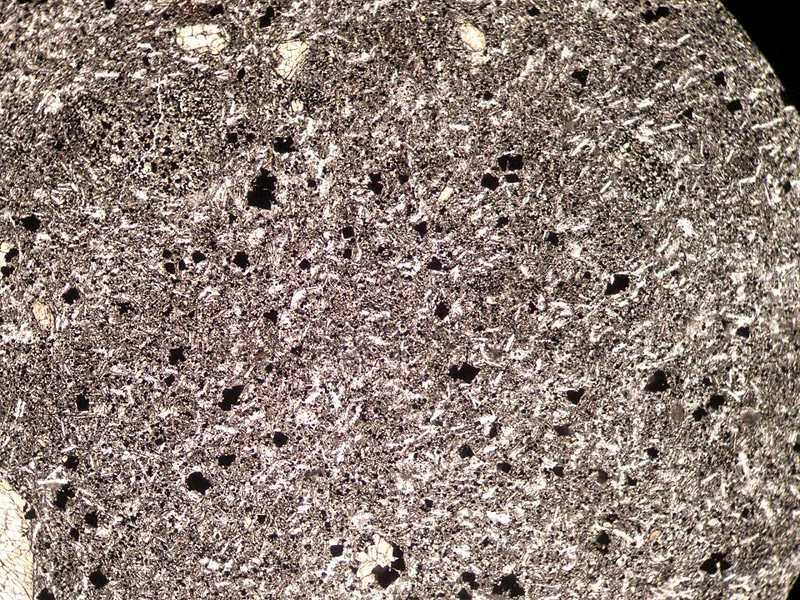
\includegraphics[height=3.6cm]{images/book2/g11-chmee2-basalt-ppl.jpg}\hfill
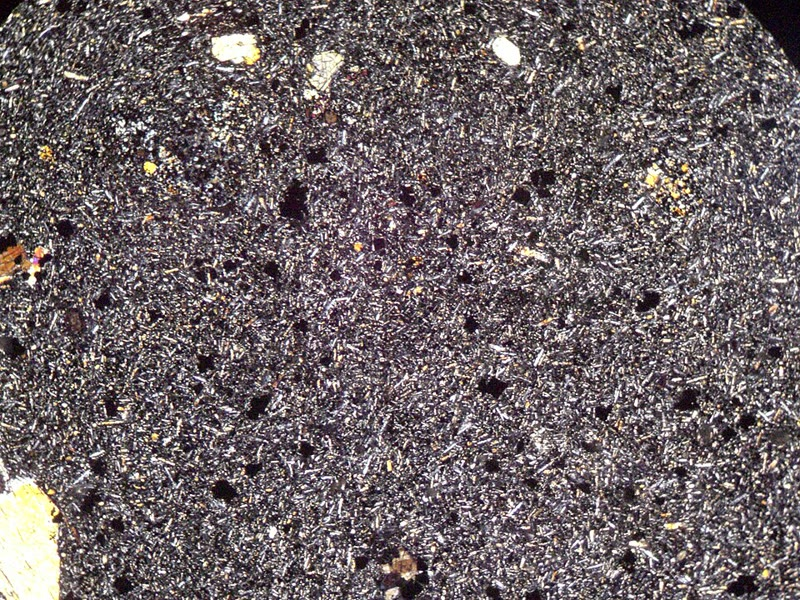
\includegraphics[height=3.6cm]{images/book2/g11-chmee2-basalt-xpl.jpg}\hfill
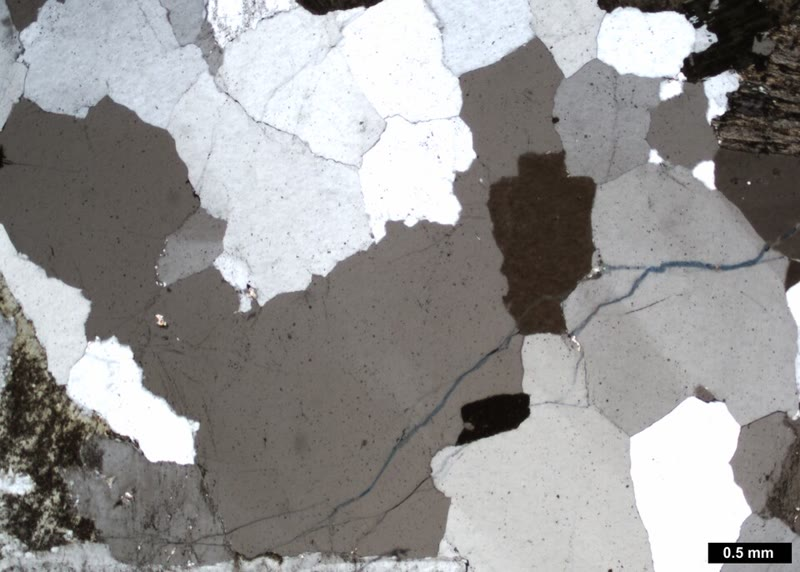
\includegraphics[height=3.6cm]{images/book2/g11-rygel-granite-xpl.jpg}

{\small Links en midden: hetzelfde basalt in \omterm{def:g11:minerals:thin-section}{slijpplaatje}, in lineair gepolariseerd
licht en tussen gekruiste polarisatoren. Het gesteente is fijnkorrelig: kleine langwerpige
kristallen, vooral plagioklaas, en zwarte stippen die in geen van beide beelden licht doorlaten;
tussen gekruiste polarisatoren lichten de kristallen op in grijstinten en
kleuren. Foto's
Chmee2 (CC~BY-SA~3.0). Rechts: kwartskristallen in een graniet, tussen
gekruiste polarisatoren, elk in een eigen grijstint (de schaalbalk is
\qty{0.5}{mm}). Foto Michael C.~Rygel (CC~BY-SA~3.0).}
\end{omfigure}
% ledger: photo:g11-basalt-thin-section, photo:g11-granite-thin-section

In lineair gepolariseerd licht lijkt een \omterm{def:g11:minerals:thin-section}{slijpplaatje} op een glas-in-loodraam:
de meeste mineralen zijn bijna kleurloos, sommige getint, en de omtrekken van de
korrels, hun \omterm{def:g11:minerals:cleavage}{splijting} en hun \omterm{def:g11:minerals:habit}{habitus} zijn scherp te zien. Tussen gekruiste
polarisatoren zouden de filters, haaks op elkaar gezet, op zichzelf geen licht
doorlaten; de meeste mineralen veranderen het licht dat erdoorheen gaat, en verschijnen
in grijstinten of in felle kleuren, die veranderen wanneer het objectglaasje wordt gedraaid.
Twee korrels van hetzelfde mineraal kunnen er verschillend uitzien, omdat elk in
zijn eigen richting is gesneden: de kwartskorrels van het graniet hierboven zijn allemaal kwarts,
in verschillende tinten. De kleuren, hoe ze veranderen en wat ze onthullen
over elk mineraal, zijn het onderwerp van het eerste universitaire jaar; hier is het
\omterm{def:g11:minerals:thin-section}{slijpplaatje} een afbeelding van het gesteente, waarin elke korrel kan worden gezien,
benoemd en geteld.

\section{Oefeningen}

\begin{exercise}[$\star$]\label{exo:g11:minerals:1}
Definieer \omterm{def:g11:minerals:cleavage}{splijting} en breuk. Welke van de twee vertoont kwarts, en hoe zien zijn
breukvlakken eruit? Hoeveel \omterm{def:g11:minerals:cleavage}{splijtrichtingen} heeft een mica?
\end{exercise}

\begin{exercise}[$\star$]\label{exo:g11:minerals:2}
Waarom is kleur een slechte gids om kwarts te identificeren, maar een vrij goede voor
olivijn? Geef twee eigenschappen die betrouwbaarder zijn dan kleur.
\end{exercise}

\begin{exercise}[$\star$]\label{exo:g11:minerals:3}
Koppel elke beschrijving aan een mineraal uit kwarts, orthoklaas, biotiet en
olivijn: (1) groene korrels in een basalt; (2) zwarte schilfers die zich in dunne
blaadjes laten afpellen; (3) roze blokvormige korrels met twee platte breukvlakken, gekrast door een
stalen spijker; (4) glazige grijze korrels met gebogen breuken, niet gekrast door de
spijker.
\end{exercise}

\begin{exercise}[$\star$]\label{exo:g11:minerals:4}
(1) Hoeveel atomen bevat een \omterm{def:g11:minerals:silicate}{silicium-zuurstoftetraëder}, en waar zitten
ze? (2) Bereken met de ladingen van de ionen \ce{Si^4+} en \ce{O^2-} de
lading van de groep \ce{SiO4}.
\end{exercise}

\begin{exercise}[$\star$]\label{exo:g11:minerals:5}
Noem de zes groepen \omterm{def:g11:minerals:rock-forming}{gesteentevormende silicaten} en geef voor elke groep de manier
waarop zijn tetraëders zijn verbonden.
\end{exercise}

\begin{exercise}[$\star\star$]\label{exo:g11:minerals:6}
De atoommassa's van silicium en zuurstof zijn \qty{28.085}{g/mol} en
\qty{15.999}{g/mol}. (1) Bereken het aandeel van zuurstof in de massa van kwarts,
\ce{SiO2}. (2) Doe hetzelfde voor forsteriet, het magnesiumolivijn
\ce{Mg2SiO4} (magnesium: \qty{24.305}{g/mol}). (3) Vergelijk met het aandeel
zuurstof in de continentale korst, ongeveer \qty{46}{\percent}.
\end{exercise}

\begin{exercise}[$\star\star$]\label{exo:g11:minerals:7}
Een witte korrel in een graniet krast een glasplaatje (ongeveer 5.5) maar wordt
gekrast door een stalen spijker (ongeveer 6.5); hij breekt langs platte vlakken in twee
richtingen. Een tweede, grijze korrel wordt niet gekrast door de spijker en breekt
langs gebogen oppervlakken. Identificeer beide, en geef de redenen.
\end{exercise}

\begin{exercise}[$\star\star$]\label{exo:g11:minerals:8}
In het pyroxeen augiet deelt elke tetraëder twee hoekpunten. (1) Hoeveel zuurstofatomen
zijn er, volgens de propositie over het tellen van de zuurstofatomen, per
silicium? (2) Controleer dat het deel \ce{(Si,Al)2O6} van de formule van augiet
daarmee klopt.
\end{exercise}

\begin{exercise}[$\star\star$]\label{exo:g11:minerals:9}
Een basalt bestaat naar volume uit \qty{55}{\percent} labradoriet (\qty{2.69}{g/cm^3}),
\qty{35}{\percent} augiet (\qty{3.4}{g/cm^3}) en \qty{10}{\percent} olivijn
(\qty{3.32}{g/cm^3}). Bereken zijn dichtheid, en dan de massa van een
kubus van dit basalt met ribben van \qty{10}{cm}.
\end{exercise}

\begin{exercise}[$\star\star$]\label{exo:g11:minerals:10}
Een \omterm{def:g11:ocean-ridges:peridotite}{peridotiet} van de mantel bestaat uit \qty{75}{\percent} olivijn
(\qty{3.32}{g/cm^3}) en \qty{25}{\percent} augiet (\qty{3.4}{g/cm^3}).
(1) Bereken zijn dichtheid. (2) Met welk percentage is hij dichter dan het
basalt van de vorige oefening, van ongeveer \qty{3.00}{g/cm^3}? (3) Waarom blijft
de \omterm{def:g11:ocean-ridges:oceanic-lithosphere}{oceanische korst} boven op de mantel liggen?
\end{exercise}

\begin{exercise}[$\star\star$]\label{exo:g11:minerals:11}
Op een \omterm{def:g11:minerals:thin-section}{slijpplaatje} van een gesteente valt een rooster van 400 punten 168 keer op
plagioklaas, 132 keer op pyroxeen, 60 keer op olivijn en 40 keer op
gaten die door gasbellen zijn achtergelaten. (1) Bereken het aandeel van elk. (2) Waarom kan de
propositie over de dichtheid van een gesteente niet direct op het hele
plaatje worden toegepast? (3) Bereken de dichtheid van het vaste deel, met \qty{2.69}{},
\qty{3.4}{} en \qty{3.32}{g/cm^3}, en dan die van het gesteente met zijn gaten.
\end{exercise}

\begin{exercise}[$\star\star\star$]\label{exo:g11:minerals:12}
In \qty{1}{kg} continentale korst zit ongeveer \qty{464}{g} zuurstof,
\qty{283}{g} silicium, \qty{84}{g} aluminium, \qty{52}{g} ijzer,
\qty{46}{g} calcium, \qty{28}{g} magnesium, \qty{23}{g} natrium en
\qty{15}{g} kalium. De atoommassa's zijn \qty{16.0}{}, \qty{28.1}{},
\qty{27.0}{}, \qty{55.8}{}, \qty{40.1}{}, \qty{24.3}{}, \qty{23.0}{} en
\qty{39.1}{g/mol}. (1) Bereken het aantal mol van elk element. (2) Welk
deel van de atomen van de korst zijn zuurstofatomen? (3) Waarom wordt de korst
soms beschreven als een stapeling van zuurstofionen, met de andere elementen in
de ruimten ertussen?
\end{exercise}

\begin{exercise}[$\star\star\star$]\label{exo:g11:minerals:13}
In een dubbele keten van een amfibool deelt de helft van de tetraëders twee hoekpunten en
de andere helft drie. (1) Hoeveel zuurstofatomen zijn er per silicium? (2) Schrijf
het resultaat voor vier siliciumatomen. (3) In de formule van hoornblende,
\ce{Ca2[Mg4(Al,Fe)]Si7AlO22(OH)2}, neemt aluminium in één op de acht tetraëders de plaats
van silicium in. Controleer dat de formule klopt.
\end{exercise}

\begin{exercise}[$\star\star\star$]\label{exo:g11:minerals:14}
Over de Sierra Nevada van Californië hebben \num{6454} granietachtige gesteentemonsters
een gemiddelde dichtheid van \qty{2.69}{g/cm^3}; die ligt boven \qty{2.7}{g/cm^3} in
het westen, en onder \qty{2.6}{g/cm^3} waar het graniet het rijkst is aan silica
en kalium. Bereken de dichtheid van een gesteente van \qty{20}{\percent} kwarts
(\qty{2.62}{g/cm^3}), \qty{10}{\percent} orthoklaas (\qty{2.56}{}),
\qty{50}{\percent} oligoklaas (\qty{2.65}{}), \qty{10}{\percent} biotiet
(\qty{3.09}{}) en \qty{10}{\percent} hoornblende (\qty{3.23}{}). Vergelijk
met het graniet uit het voorbeeld van dit hoofdstuk, en verklaar het contrast
tussen de twee delen van de Sierra Nevada.
\end{exercise}

\begin{exercise}[$\star\star\star$]\label{exo:g11:minerals:15}
De bovenste continentale korst bevat naar massa ongeveer \qty{66.6}{\percent} \ce{SiO2},
de continentale korst als geheel \qty{60.6}{\percent}. (1) Bereken met
het aandeel silicium in \ce{SiO2} (\qty{46.7}{\percent}) het aandeel
silicium dat in elk ervan in \ce{SiO2} vastligt. (2) Welke mineralen zou je verwachten
die in de bovenkorst vaker voorkomen dan dieper? (3) Wat betekent dit
voor de dichtheid van de bovenkorst vergeleken met de diepere korst?
\end{exercise}

\section{Probleem: de dichtheid van een graniet}

\begin{problem}[{Weekendprobleem --- van een puntentelling naar een dichtheid}]
\label{pb:g11:minerals:1}
% values (mineral_density.py): GRANITE_COUNT 150/175/125/30/20; rho_granite 2.6427;
% granite_air_g 264.27, granite_water_g 164.27; densities wm:densities; usgs91:sierra
Een blok roze graniet wordt gezaagd en gepolijst. Zijn mineralen worden geïdentificeerd,
op een rooster geteld, en de dichtheid van het gesteente wordt berekend, en dan door
weging gecontroleerd.

\medskip
\noindent\textbf{Deel I --- De mineralen identificeren.}
\begin{enumerate}
  \item Korrels A zijn grijs en glazig, tonen geen plat breukvlak, alleen
        gebogen, en worden niet gekrast door een stalen spijker. Welk mineraal
        zijn het?
  \item Korrels B zijn roze en blokvormig, breken langs platte glanzende vlakken in
        twee richtingen, krassen glas maar worden gekrast door de spijker. Welk
        mineraal zijn het, en wat is hun hardheid op de schaal van Mohs?
  \item Korrels C hebben dezelfde hardheid en \omterm{def:g11:minerals:cleavage}{splijting} als korrels B maar zijn
        wit; een analyse vindt er natrium en calcium in, en geen
        kalium. Welk soort veldspaat zijn het?
  \item Korrels D zijn zwarte schilfers, korrels E zilverige schilfers; beide laten zich in
        dunne blaadjes afpellen. Welke mineralen zijn het, en welk kenmerk van hun
        structuur verklaart de blaadjes?
  \item Welke van de mineralen A tot E zijn raamwerksilicaten? Welke bevatten
        ijzer en magnesium?
\end{enumerate}

\medskip
\noindent\textbf{Deel II --- De puntentelling.}
\begin{enumerate}[resume]
  \item Een rooster van 500 punten valt 150 keer op kwarts, 175 keer op
        orthoklaas, 125 keer op oligoklaas, 30 keer op biotiet en 20 keer
        op muscoviet. Bereken het aandeel van elk mineraal.
  \item Waarom schat het aandeel van de punten het aandeel van het volume
        van het gesteente?
  \item Welk percentage van het gesteente is veldspaat?
  \item Als één punt verkeerd wordt geteld, hoeveel verandert een aandeel dan?
  \item Is dit gesteente een graniet in de zin van Boek 1?
\end{enumerate}

\medskip
\noindent\textbf{Deel III --- De dichtheid.}
\begin{enumerate}[resume]
  \item Geef de formule voor de dichtheid van een gesteente zonder poriën uit
        zijn mineralen.
  \item Bereken met de dichtheden kwarts \qty{2.62}{}, orthoklaas \qty{2.56}{},
        oligoklaas \qty{2.65}{}, biotiet \qty{3.09}{} en muscoviet
        \qty{2.82}{g/cm^3} de bijdrage $\phi_i \rho_i$ van
        elk mineraal.
  \item Tel ze op: wat is de dichtheid van het graniet?
  \item Welk mineraal draagt het meest bij aan de som? Welke twee mineralen
        verhogen zijn dichtheid, hoewel ze maar een tiende van het gesteente uitmaken?
  \item Reken de dichtheid om naar \unit{kg/m^3}, en geef de massa van
        \qty{1}{m^3} van dit graniet.
\end{enumerate}

\medskip
\noindent\textbf{Deel IV --- Controle door weging.}
\begin{enumerate}[resume]
  \item Uit het graniet wordt een blok van \qty{100}{cm^3} gezaagd. Welke massa
        verwacht je?
  \item Een lichaam dat in water hangt, wordt omhooggeduwd door het gewicht van het water dat het
        verplaatst (natuurkunde). Welke massa leest de balans af wanneer het blok
        helemaal ondergedompeld hangt in water met dichtheid \qty{1.00}{g/cm^3}?
  \item Laboratoria berekenen de dichtheid van een gesteentemonster als
        $m_{\text{lucht}}/(m_{\text{lucht}} - m_{\text{water}})$. Controleer dat
        je twee massa's de dichtheid van vraag~13 teruggeven.
  \item Granietachtige gesteenten van de Sierra Nevada hebben gemiddeld \qty{2.69}{g/cm^3}, en
        die het rijkst aan silica en kalium liggen onder \qty{2.6}{g/cm^3}.
        Waar ligt dit graniet, en welke mineralen zouden een
        graniet dichter maken?
  \item Besluit: wat is de dichtheid van het graniet?
\end{enumerate}
\end{problem}
